%----------------------------------------------------------------------------
%----------------------------------------------------------------------------
%----------------------------------------------------------------------------
%----------------------------------------------------------------------------
Given an arbitrary pulse width of $\sigma_{\alpha}=2$, we seek to find the pulse height $A$ that corresponds to a complete inversion (gound state complete depleted). Suppose the solution, $\ket{\Psi}$, to (\ref{one dynamics}) is known. Consider the cost function
%----------------------------------------------------------------------------
\begin{equation}
\Phi
=
P_0(t=t_{final})
\label{one cost}
\end{equation}
%----------------------------------------------------------------------------
where $P_0$ be the probability that the system is found in the ground state (i.e. $\braket{0}{0}$); thus, if $P_0=0$ then the two level system is completely inverted.
%----------------------------------------------------------------------------
%----------------------------------------------------------------------------
A MathCAD program is used to minimize (\ref{one cost}) as a function of $A$ for a system initially in the ground state over the time interval $[0,30]$ (thus Equation \ref{one cost} is evaluated at $t=30$). A fourth-order Runge-Kutta fixed-step method is used to find the solution at 5000 points in the time interval. The MathCAD function ``Minimize'' is used to find the optimal solution. The ``Minimize'' function tries the conjugate gradient, quasi-Newton, and Levenberg-Marquardt methods in succession until one converges.

Figure \ref{solution one} shows the pulse and resulting motion in $\braket{\Phi}{\Phi}$ at a local optimum. There are many local optima as one increases $A$. The nature of these repeated optima becomes obvious when one considers the analytic solution (they are sucessive Rabi oscillations), Equation \ref{2 level dynamics}; in lieu of such a discussion we present an example (see figure \ref{big solution one}).
%----------------------------------------------------------------------------
%----------------------------------------------------------------------------
% solution_1.tex
% by Troy Hix, April 2005
%----------------------------------------------------------------------------
\begin{figure}
\centering
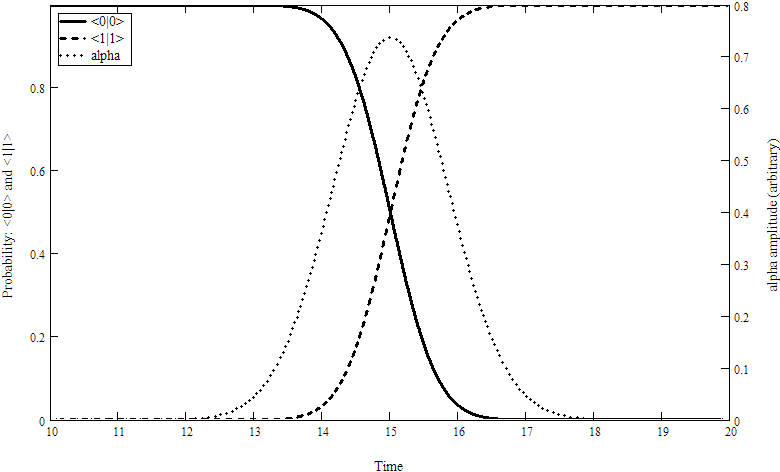
\includegraphics[width=5.00in]
{solution_1/solution_1.png}\\
\caption[Single color optimal solution]{Single color optimal solution. With $\sigma_{\alpha}\equiv 2$, this local optimum occurs when $A=0.737832313319$. Many more local optima occur with increasing $A$. If the pulse area is $\xi$, then $\xi - \pi/2 \sim 10^{-12}$ (the precision of $A$). In the literature, this is called a $\pi$--pulse.}
\label{solution one}
\end{figure} 
%----------------------------------------------------------------------------

%----------------------------------------------------------------------------
%----------------------------------------------------------------------------
% big_solution_1.tex
% by Troy Hix, April 2005
%----------------------------------------------------------------------------
\begin{figure}
\centering
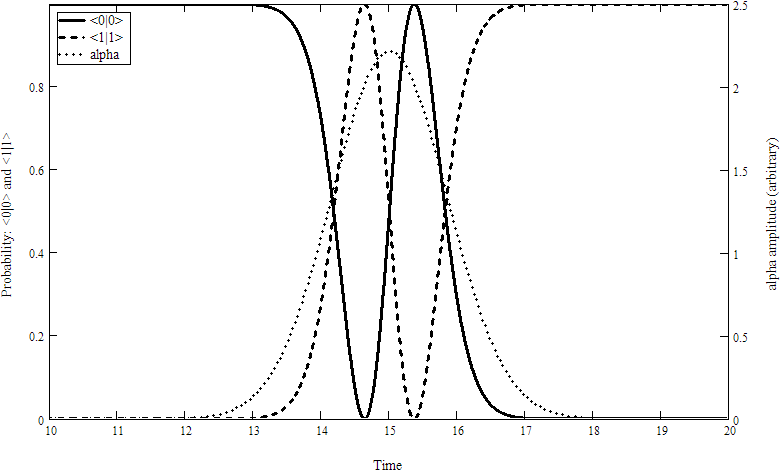
\includegraphics[width=5.00in]
{big_solution_1/big_solution_1.png}\\
\caption[Single color optimal solution - increased pulse amplitude]{Single color optimal solution - increased pulse amplitude. This local optimum occurs when $A=3\cross0.737832313319$ (three times the area of the $\pi$--pulse).}
\label{big solution one}
\end{figure} 
%----------------------------------------------------------------------------

%----------------------------------------------------------------------------
%----------------------------------------------------------------------------
%----------------------------------------------------------------------------
%----------------------------------------------------------------------------
